\documentclass[tikz,border=10pt]{standalone}
\usetikzlibrary{arrows.meta, positioning, calc, decorations.pathreplacing}
\usepackage{amssymb}

\begin{document}
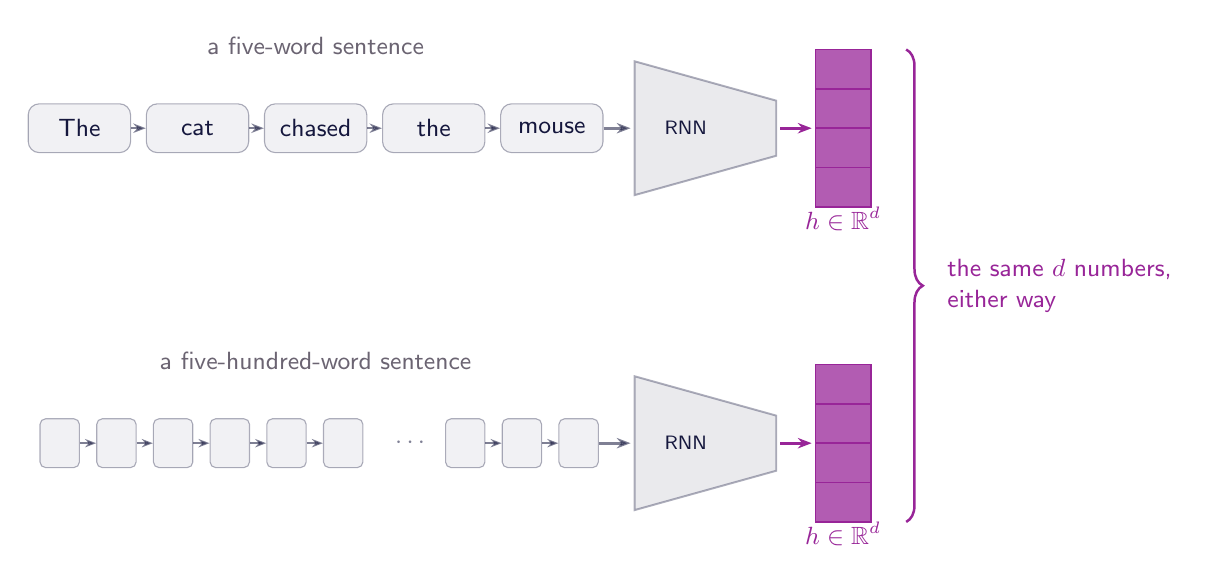
\begin{tikzpicture}[
    every node/.style={font=\sffamily},
]

% ---------------------------------------------------------------- colours
\definecolor{c1}{HTML}{15173D}   % structure, tokens, the recurrent network
\definecolor{c2}{HTML}{982598}   % the bottleneck vector, the operative object
\definecolor{c3}{HTML}{E491C9}
\definecolor{c4}{HTML}{F1E9E9}
\definecolor{axiscolor}{HTML}{333333}
\definecolor{labelcolor}{HTML}{6B6472}

% ---------------------------------------------------------------- styles
\tikzset{
    word/.style={
        rectangle, rounded corners=4pt, minimum width=1.3cm,
        minimum height=0.62cm, inner xsep=4pt,
        draw=c1, draw opacity=0.35, fill=c1, fill opacity=0.06,
        text=c1, text opacity=1, font=\sffamily\small,
    },
    tick/.style={
        rectangle, rounded corners=2pt, minimum width=0.5cm,
        minimum height=0.62cm,
        draw=c1, draw opacity=0.35, fill=c1, fill opacity=0.06,
    },
    cell/.style={
        rectangle, minimum width=0.7cm, minimum height=0.5cm,
        draw=c2, line width=0.6pt, fill=c2, fill opacity=0.75,
    },
}

% ================================================================
% GEOMETRY
%   row A (short sentence)  centred on y = 5.5
%   row B (long sentence)   centred on y = 1.5
%   tokens        x in [0.3, 7.4]
%   funnel        x in [7.9, 9.7]
%   state vector  x in [10.2, 10.9]
%   brace         x  = 11.6
% ================================================================

% ---------------------------------------------------------------- row A
\node[font=\sffamily\small, text=labelcolor] at (3.85, 6.55)
    {a five-word sentence};

\node[word] (a1) at (0.85, 5.5) {The};
\node[word] (a2) at (2.35, 5.5) {cat};
\node[word] (a3) at (3.85, 5.5) {chased};
\node[word] (a4) at (5.35, 5.5) {the};
\node[word] (a5) at (6.85, 5.5) {mouse};

\foreach \i/\j in {a1/a2, a2/a3, a3/a4, a4/a5} {
    \draw[-{Stealth[length=4.5pt]}, line width=0.9pt, c1, opacity=0.55]
        (\i) -- (\j);
}

% funnel: everything read so far is compressed into one state
\fill[c1, opacity=0.09]
    (7.9, 6.35) -- (9.7, 5.85) -- (9.7, 5.15) -- (7.9, 4.65) -- cycle;
\draw[c1, opacity=0.35, line width=0.7pt]
    (7.9, 6.35) -- (9.7, 5.85) -- (9.7, 5.15) -- (7.9, 4.65) -- cycle;
\node[font=\sffamily\scriptsize, text=c1] at (8.55, 5.5) {RNN};

\draw[-{Stealth[length=5pt]}, line width=1.0pt, c1, opacity=0.55]
    (a5.east) -- (7.85, 5.5);

% the fixed-size state
\foreach \k in {0,...,3} {
    \node[cell] at (10.55, 6.25 - \k*0.5) {};
}
\node[font=\sffamily\small, text=c2] at (10.55, 4.35) {$h \in \mathbb{R}^{d}$};

\draw[-{Stealth[length=5pt]}, line width=1.0pt, c2]
    (9.75, 5.5) -- (10.15, 5.5);

% ---------------------------------------------------------------- row B
\node[font=\sffamily\small, text=labelcolor] at (3.85, 2.55)
    {a five-hundred-word sentence};

\foreach \k in {0,...,5} {
    \node[tick] (b\k) at (0.6 + \k*0.72, 1.5) {};
}
\node[font=\sffamily\small, text=c1, opacity=0.55] at (5.05, 1.5) {$\cdots$};
\foreach \k in {0,...,2} {
    \node[tick] (d\k) at (5.75 + \k*0.72, 1.5) {};
}

\foreach \i/\j in {b0/b1, b1/b2, b2/b3, b3/b4, b4/b5} {
    \draw[-{Stealth[length=4pt]}, line width=0.9pt, c1, opacity=0.55]
        (\i) -- (\j);
}
\foreach \i/\j in {d0/d1, d1/d2} {
    \draw[-{Stealth[length=4pt]}, line width=0.9pt, c1, opacity=0.55]
        (\i) -- (\j);
}

\fill[c1, opacity=0.09]
    (7.9, 2.35) -- (9.7, 1.85) -- (9.7, 1.15) -- (7.9, 0.65) -- cycle;
\draw[c1, opacity=0.35, line width=0.7pt]
    (7.9, 2.35) -- (9.7, 1.85) -- (9.7, 1.15) -- (7.9, 0.65) -- cycle;
\node[font=\sffamily\scriptsize, text=c1] at (8.55, 1.5) {RNN};

\draw[-{Stealth[length=5pt]}, line width=1.0pt, c1, opacity=0.55]
    (d2.east) -- (7.85, 1.5);

\foreach \k in {0,...,3} {
    \node[cell] at (10.55, 2.25 - \k*0.5) {};
}
\node[font=\sffamily\small, text=c2] at (10.55, 0.35) {$h \in \mathbb{R}^{d}$};

\draw[-{Stealth[length=5pt]}, line width=1.0pt, c2]
    (9.75, 1.5) -- (10.15, 1.5);

% ---------------------------------------------------------------- the point
\draw[decorate, decoration={brace, amplitude=6pt}, c2, line width=0.9pt]
    (11.35, 6.5) -- (11.35, 0.5);
\node[font=\sffamily\small, text=c2, anchor=west, align=left]
    at (11.75, 3.5) {the same $d$ numbers,\\either way};

\end{tikzpicture}
\end{document}
